% !TeX root = ../HebutThesis_example.tex(此文件是被HebutThesis_example.tex调用的)

\chapter{基础知识}
\section{数学}

\subsection{线性代数}
\subsubsection{对角矩阵}
除主对角线之外的元素皆为{$0$}的矩阵。

\subsubsection{矩阵乘法}
如果{$A$}是一个{$l\times m$}矩阵,
{$B$}是一个{$m\times n$}矩阵,
则{$AB$}是一个{$l\times n$}矩阵。

\subsubsection{矩阵的迹}
矩阵的迹为矩阵所有对角元素之和,即:
\begin{equation}
    \label{eq:matrix_trac}
    Tr(A)=\sum_{i}A_{i,i}
\end{equation}

\subsubsection{范数}
范数可以表示向量的大小,范数定义为:
\begin{equation}
    \label{eq:norm}
    {\Vert \bm{x} \Vert}_{p} = {\left(  \sum_{i} \mid x_i  \mid^p    \right)}^{\frac{1}{p}}
\end{equation}
式{\ref{eq:norm}}中,{$p \in \mathbb{R}, p\geq 1$}

{$L^1$}范数为:
\begin{equation}
    \label{eq:l1_norm}
    \Vert \bm{x} \Vert_{1} =  \sum_{i} \mid x_i \mid
\end{equation}

最大范数为:
\begin{equation}
    \label{eq:max_norm}
    \Vert \bm{x} \Vert_{\infty} = \max_i \mid x_i \mid
\end{equation}


矩阵的Frobenius范数为:
\begin{equation}
    \label{eq:frobenius_norm}
    \Vert \bm{x} \Vert_{F} =\sqrt{\sum_{i,j}A_{i,j}^{2}}=\sqrt{Tr(AA^{T})}
\end{equation}

\subsubsection{矩阵行列式}
矩阵的行列式是一个关于方形矩阵(方阵)内所有元素的标量函数值。
一个{$n\times n$}的矩阵{$M$}的行列式为:
\begin{equation}
    \label{eq:determinant_of_matrix}
    \det M =\det
    \begin{bmatrix}
        a_{11}&a_{12}&\cdots &a_{1n} \\
        a_{21}&a_{22}&\cdots &a_{2n} \\
        \vdots & \vdots & & \vdots \\
        a_{n1}&a_{n2}&\cdots &a_{nn}
    \end{bmatrix}
    =\sum_{j_1j_2\cdots j_n}{(-1)}^{\tau (j_1j_2\cdots j_n)}a_{1j_1}a_{2j_2}\ldots a_{nj_n}
\end{equation}

式{\ref{eq:determinant_of_matrix}}中,
求和符号{$\sum $}的下标{$j_1j_2\cdots j_n$}表示集合{$1,2,\ldots ,n$}的全排列,
即共有{$n\!$} 项;
{$\tau({j_1j_2\cdots j_n})$}表示排列{$j_1j_2\cdots j_n$}的符号,
排列的符号定义为式{\ref{eq:parity_of_a_permutation}}。

方阵的行列式可以用来判断矩阵{$M$}是否可逆:
如果{$\det M = 0$},那么矩阵不可逆。

矩阵乘积的行列式等于矩阵行列式的乘积,即:
\begin{equation}
    \det (AB)=\det(A)\det(B)
\end{equation}

\subsubsection{可逆矩阵}
如果一个{$n \times n$}的矩阵{$A$}可逆,那么存在{$n \times n$}矩阵{$B$}使得:
\begin{equation}
    \label{eq:invertable_matrix_defination}
    AB=BA=I_n
\end{equation}

式{\ref{eq:invertable_matrix_defination}}中,{$I_n$}为单位矩阵,并且使用矩阵乘法。

不可逆的方阵又称为奇异矩阵或退化矩阵。

对于可逆矩阵有:
\begin{equation}
    \det(M)\det(M^{-1})=\det(M\dot M^{-1})
    =\det(I)=1
\end{equation}
因此,
\begin{equation}
    \label{eq:determinant_of_inverse_matrix}
    \det (M^{-1})={(\det(M))}^{-1}
\end{equation}




\subsubsection{雅可比矩阵}

假设某函数{$\bm{f}:\mathbb{R}^{n}\rightarrow\mathbb{R}^{m}$},
从{$\bm{x}\in\mathbb{R}^{n}$}映射到向量{$\bm{f(x)}\in\mathbb{R}^{m}$},
这个函数的一阶偏导矩阵称为雅可比矩阵,是一个{$m\times n$}的矩阵。
其第{$i$}行,第{$j$}列的值为{$\bm{J}_{ij}=\frac{\partial f_i}{\partial x_i} $}
\begin{equation}
    \label{eq:jacabian_matrix}
    \bm{J}=
    \begin{bmatrix}
        \frac{\partial f_1}{\partial x_1}& \cdots & \frac{\partial f_1}{\partial x_n}\\
        \vdots &\ddots  & \vdots \\
        \frac{\partial f_m}{\partial x_1}& \cdots & \frac{\partial f_m}{\partial x_n}
    \end{bmatrix}
\end{equation}









\subsection{概率论}
\subsubsection{概率密度函数}
一个连续随机变量{$X$}的概率可以由概率密度函数表示:
\begin{equation}
    p(X\in A )= \int_A f_{\bm{X}}(x)dx
\end{equation}
\subsubsection{概率质量函数}
一个离散随机变量{$X$}的概率可以由概率质量函数表示:
\begin{equation}
    p_{X}(x)=p(\{X=x\})
\end{equation}
\subsubsection{正态分布}
若实值随机变量{$X$}服从正态分布(高斯分布),
则其概率密度函数为:
\begin{equation}
    \label{eq:gaussian_distribution}
    f(x)=\frac{1}{\sigma\sqrt{2\pi}}\exp({\frac{1}{2}{(\frac{x-\mu}{\sigma})}^{2}})
\end{equation}
记为:{$X\sim \mathcal{N}(\mu,\sigma^{2})$}

两高斯分布之和仍为高斯分布,
假设{$X,Y$}为两独立随机变量,
且
\begin{align}
    X\sim & \mathcal{N}(\mu_X,\sigma_{X}^{2}) \\ 
    Y\sim & \mathcal{N}(\mu_Y,\sigma_{Y}^{2}) \\
\end{align}
则{$X,Y$}之和仍为高斯分布,
即:
\begin{align}
    Z=&X+Y\\
    Z\sim& \mathcal{N}(\mu_X+\mu_Y,\sigma_{X}^{2}+\sigma_{Y}^{2})  \label{eq:sum_of_two_gaussian_distributions}
\end{align}

\subsubsection{期望}
当{$x \sim p(x)$},函数{$f(x)$}的期望为:
\begin{equation}
    \label{eq:expection_discrete}
    \mathbb{E}_{x \sim p} [ f(x)] = \sum_{x} p(x)f(x)
\end{equation}
或
\begin{equation}
    \label{eq:expection_continuous}
    \mathbb{E}_{x \sim p} [ f(x)] = \int p(x)f(x) \,dx
\end{equation}

\subsubsection{协方差}
随机变量{$X,Y$}的协方差为:
\begin{equation}
    \label{eq:covariance}
    cov(X,Y)=\mathbb{E}\left[XY\right]-\mathbb{E}\left[X\right]\mathbb{E}\left[Y\right]
\end{equation}


\subsubsection{极大似然估计}

假设{$\theta$}为未知参数(标量或者矢量),
对于服从联合概率质量函数{$p_{X}(\bm{x};\theta)$}的一组观测向量{$X={X_1,\ldots,X_n}$},
假设我们有{$X$}的具体的观测值{$\bm{x}=(x_1,\ldots,x_n)$}。
那么,其极大似然估计是未知参数{$\theta$}的一个取值,
该取值能够使函数{$p_{X}(x_1,\ldots,x_n;\theta)$}取得最大值。
\begin{equation}
    \label{eq:maximux_likelihood_estimation_orgin}
    \hat{\theta_n}
    =\argmax_{\theta} p_X(\bm{x};\theta)
    =\argmax_{\theta} p_X(x_1,\ldots,x_n;\theta)
\end{equation}



\begin{figure}[ht]
    \centering
    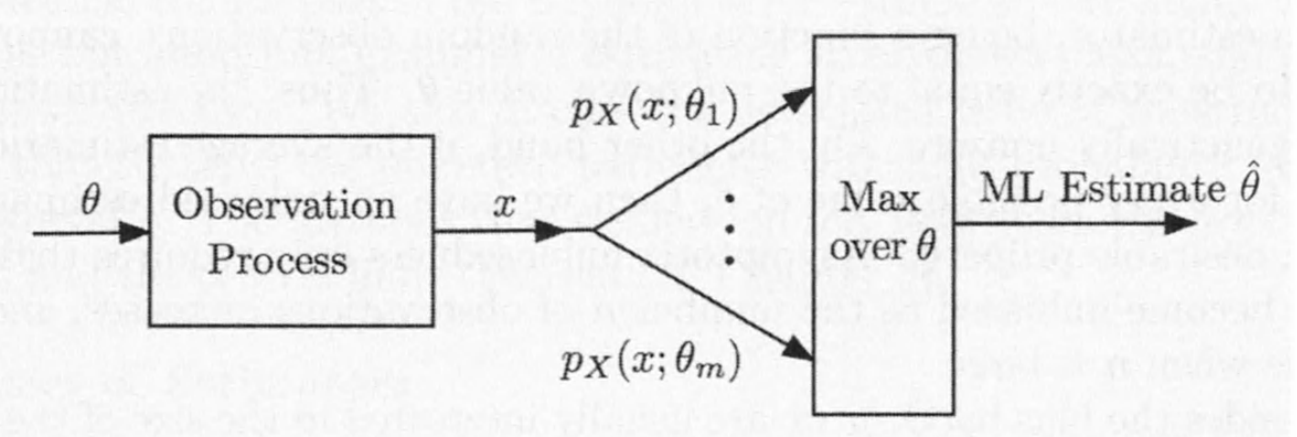
\includegraphics[width=0.8\textwidth]{figures/maximux_likelihood_estimation}
    \caption{极大似然估计示意图}\label{fig:maximux_likelihood_estimation}
\end{figure}

图{\ref{fig:maximux_likelihood_estimation}}中,
假设{$X$}为离散变量,
未知参数{$\theta$}可以从{$\theta_1,\ldots,\theta_m$}中选取。
给定观测值{$X=\bm{x}$},
对于每个{$\theta_i$}取值,
都可以计算{$p_X(\bm{x};\theta_i)$}。
使函数{$p_X(\bm{x};\theta)$}取得最大值的{$\theta_i$}即为极大似然估计{$\theta$}。

在很多情况下,都假定观测向量中的每一个{$X_i$}为互相独立的,
因此,似然函数通常可以改写为:
\begin{equation}
    \label{eq:maximux_likelihood_estimation_discrete}
    p_X(x_1,\ldots,x_n;\theta)=\prod_{i=1}^{n}p_{X_i}(x_i;\theta)
\end{equation}

为了分析与计算方便,可以将其改写为对数似然函数:
\begin{equation}
    \label{eq:maximux_likelihood_estimation_discrete_log}
    \log p_X(x_1,\ldots,x_n;\theta)
    =\log \prod_{i=1}^{n}p_{X_i}(x_i;\theta) 
    =\sum_{i=1}^{n} \log p_{X_i}(x_i;\theta)
\end{equation}

当{$X$}为连续变量时,由概率密度函数替换概率质量函数可得:
\begin{equation}
    \label{eq:maximux_likelihood_estimation_continuous_log}
    \log f_X(x_1,\ldots,x_n;\theta)
    =\log \prod_{i=1}^{n}f_{X_i}(x_i;\theta) 
    =\sum_{i=1}^{n} \log f_{X_i}(x_i;\theta)
\end{equation}

值得注意的是,
对于{$X$}的观测值{$\bm{x}$},
其似然函数{$p_X(\bm{x};\theta)$}并不是指未知 参数取值为{$\theta$}的概率,
而是指在未知参数取值为{$\theta$}时,
{$X$}的观测值为{$\bm{x}$}的概率。

\subsubsection{边缘似然}
边缘似然是似然函数在参数空间上的积分,
表示生成观测样本的概率,
因此,边缘似然也被称为模型证据,简称为证据。




\subsubsection{全概率公式}

全概率公式将对一复杂事件A的概率求解问题转化为了在不同情况下发生的简单事件的概率的求和问题。

若事件{$B_1,B_2,\dots,B_n$}构成一个完备事件组且都有正概率,则有,
\begin{align}
    p(A)
    & =p(AB_1)+p(AB_2)+ \cdots +p(AB_n) \label{eq:total_probability_theorem_1}\\
    & =p(A|B_1)p(B_1)+p(A|B_2)p(B_2)+ \cdots + p(A|B_n)p(B_n) \label{eq:total_probability_theorem_2}
\end{align}




\subsubsection{贝叶斯定理}
若事件{$B_1,B_2,\dots,B_n$}构成一个完备事件组且都有正概率,则有,
\begin{align}
    p(B_i|A)
    & =\frac{p(A|B_i)p(B_i)}{p(A)} \label{eq:bayes_rule_1}\\
    & =\frac{p(A|B_i)p(B_i)}{p(A|B_1)p(B_1)+p(A|B_2)p(B_2)+ \cdots +p(A|B_n)p(B_n)} \label{eq:bayes_rule_2}
\end{align}

在式{\ref{eq:bayes_rule_1}}与{\ref{eq:bayes_rule_2}}中,
{$B_i$}通常表示一个命题,如“硬币正面朝上的次数占投掷次数的50\%”;
{$A$}通常表示事实,如“连续多次投掷硬币的结果”。
{$p(B_i)$}表示{$B_i$}的先验概率,
先验概率为不考虑事实{$A$}时,
人们对事件{$B_i$}的相信程度,
其也包含了人们对于{$B_i$}的先验知识。
{$p(A|B_i)$}为似然函数,
表示当命题{$B_i$}发生时,
事实{$A$}发生的概率。
“似然”表达了事件{$A$}对命题{$B_i$}的支撑程度。
{$p(B_i|A)$}为{$B_i$}的后验概率,
表示考虑事实{$A$}后,
命题{$B_i$}发生的概率。
贝叶斯定理根据事实{$B_i$},
对先验概率{$p(B_i)$}进行更新。

\subsubsection{贝叶斯推理}
贝叶斯推理可以由先验概率和似然函数得出后验概率,
其中先验概率和似然函数皆由统计模型关于观测数据产生。
\begin{equation}
    \label{eq:bayesian_inference}
    p(H\mid E)=\frac{p(E \mid H)p(H)}{p(E)}
\end{equation}
式{\ref{eq:bayesian_inference}}中:
\begin{itemize}
    \item {$H$}为假设,其概率受数据(以下称为证据)影响。
    \item {$p(H)$}为先验概率,是在获得数据{$E$}前,对假设{$H$}概率的估计,{$E$}为当前证据。
    \item {$E$}为证据,即未参与先验概率{$p(H)$}计算的数据。
    \item {$p(H\mid E)$}未后验概率,给出证据{$E$}后,{$H$}为真的概率,是关于{$H$}的函数。
    \item {$p(E\mid H)$}为似然函数,给出假设{$H$}后观测到{$E$}的概率,是关于{$E$}的函数。
    \item {$p(E)$}为边缘似然,也称为模型证据。表示从先验概率中获得观测样本的概率。
\end{itemize}


\subsubsection{蒙特卡洛方法}

蒙特卡洛方法是依赖于随机采样来获得数值结果的一种计算方法。
其底层思想是,用随机方法来解决原理上具备确定性的问题。
在物理和数学上,当其他方法不可用时,常常采用蒙特卡洛方法。
蒙特卡洛方法主要应用于三类问题:优化、数值积分与从概率分布中采样。

当无法精确求和或者计算积分时,
通常使用蒙特卡洛采样方法来近似。
基本思想为,将其和或者积分视为某分布的期望,
通过相应的计算来近似该期望。
如:
\begin{equation}
    \label{eq:monte_carlo_sampling_sum}
    s=\sum_{\bm{x}} p(\bm{x})f(\bm{x})=E_p[f(\bm{x})]
\end{equation}
\begin{equation}
    \label{eq:monte_carlo_sampling_integral}
    s=\int  p(\bm{x})f(\bm{x}) \,d\bm{x}=E_p[f(\bm{x})]
\end{equation}

式{\ref{eq:monte_carlo_sampling_sum}}中,
{$p(\bm{x})$}为随机变量{$\bm{x}$}的概率分布,
式{\ref{eq:monte_carlo_sampling_integral}}中,
{$p(\bm{x})$}为随机变量{$\bm{x}$}的概率密度。

\subsubsection{随机微分方程}
随机微分方程(Stochastic differential equation)是添加了一项或多项随机项的微分方程。



\subsubsection{对比散度}

用函数{$f(x;\bm{\theta})$}来为数据点的概率分布建模,
其中,
{$x$}为模型的输入,
{$\bm{\theta}$}为模型的参数,
且要保证概率积分为1的性质,即:
\begin{equation}
    \label{eq:contrastive_divergence_evidence_p}
    p(x;\bm{\theta})=\frac{f(x;\bm{\theta})}{Z(\bm{\theta})}
\end{equation}
式{\ref{eq:contrastive_divergence_evidence_p}}中,
{$Z(\bm{\theta})$}为划分函数:
\begin{equation}
    \label{eq:contrastive_divergence_evidence_z}
    Z(\bm{\theta})=\int f(x;\bm{\theta}) \,dx
\end{equation}
假定数据点集合为{$\bm{x}=x_1, \ldots, x_K$},
则其似然函数为:
\begin{equation}
    \label{eq:contrastive_divergence_likelihood}
    p(\bm{x};\bm{\theta})=\prod_{k=1}^{K} \frac{f(x_k;\bm{\theta})}{Z(\bm{\theta})}
\end{equation}
极大化似然函数{\ref{eq:contrastive_divergence_likelihood}}等价于最小化负对数似然函数,
即能量函数{$E(\bm{x};\bm{\theta})$}:
\begin{equation}
    \label{eq:contrastive_divergence_energy_function}
    E(\bm{x};\bm{\theta})
    = \log Z(\bm{\theta}) - \frac{1}{K} \sum_{i=1}^{K} \log f(x_i;\bm{\theta})
\end{equation}
对式{\ref{eq:contrastive_divergence_energy_function}}关于参数{$\bm{\theta}$}求偏导,
即:
\begin{align}
    \frac{\partial E(\bm{x};\bm{\theta})}{\partial \bm{\theta}}
    &= \frac{\partial  \log Z(\bm{\theta}) }{\partial \bm{\theta}} -  \frac{1}{K}  \sum_{i=1}^{K} \frac{\partial \log f(x_i;\bm{\theta})}{\partial \bm{\theta}} \\
    &= \frac{\partial  \log Z(\bm{\theta}) }{\partial \bm{\theta}} - \mathbb{E}_{p_{data}}  \left [ \frac{\partial \log f(x;\bm{\theta})}{\partial \bm{\theta}} \right ] \\
    &= \frac{1}{Z(\bm{\theta})} \frac{\partial  Z(\bm{\theta}) }{\partial \bm{\theta}} - \mathbb{E}_{p_{data}}  \left [ \frac{\partial \log f(x;\bm{\theta})}{\partial \bm{\theta}} \right ] \\
    &= \frac{1}{Z(\bm{\theta})}  \frac{\partial  \int f(x;\bm{\theta}) \,dx }{\partial \bm{\theta}}     - \mathbb{E}_{p_{data}}  \left [ \frac{\partial \log f(x;\bm{\theta})}{\partial \bm{\theta}} \right ] \\
    &=  \frac{1}{Z(\bm{\theta})} \int \frac{\partial   f(x;\bm{\theta})  }{\partial \bm{\theta}}   \,dx    - \mathbb{E}_{p_{data}}  \left [ \frac{\partial \log f(x;\bm{\theta})}{\partial \bm{\theta}} \right ] \\
    &=   \frac{1}{Z(\bm{\theta})} \int  f(x;\bm{\theta})  \frac{\partial \log  f(x;\bm{\theta}) }{\partial \bm{\theta}}   \,dx     - \mathbb{E}_{p_{data}}  \left [ \frac{\partial \log f(x;\bm{\theta})}{\partial \bm{\theta}} \right ] \\
    &=  \int  p(x;\bm{\theta})  \frac{\partial \log  f(x;\bm{\theta}) }{\partial \bm{\theta}}   \,dx    - \mathbb{E}_{p_{data}}  \left [ \frac{\partial \log f(x;\bm{\theta})}{\partial \bm{\theta}} \right ] \\
    &=   \mathbb{E}_{p(x;\bm{\theta})} \left [      \frac{\partial \log  f(x;\bm{\theta}) }{\partial \bm{\theta}}      \right ]   - \mathbb{E}_{p_{data}}  \left [ \frac{\partial \log f(x;\bm{\theta})}{\partial \bm{\theta}} \right ] \label{eq:contrastive_divergence_partial_negative_log_likelihood}
\end{align}
式{\ref{eq:contrastive_divergence_partial_negative_log_likelihood}}即为对比散度的梯度,
对于其等号右侧第一项
\begin{equation}
    \mathbb{E}_{p(x;\bm{\theta})} \left [      \frac{\partial \log  f(x;\bm{\theta}) }{\partial \bm{\theta}}      \right ]
\end{equation}
可以通过多次循环使用马尔科夫链蒙特卡洛采样来将训练集数据转化为从{$p(x;\bm{\theta})$}分布中的采样。
假设{$\bm{x}^{n}$}表示对训练样本数据{$\bm{x}$}使用{$n$}次马尔科夫链蒙特卡洛采样获得数据,
可令{$\bm{x}^{0}=\bm{x}$},
即得:
\begin{equation}
    \label{eq:contrastive_divergence_gradient_mcmc_infinite}
    \frac{\partial E(\bm{x};\bm{\theta})}{\partial \bm{\theta}}
    =   \mathbb{E}_{\bm{x}^{\infty}} \left [      \frac{\partial \log  f(x;\bm{\theta}) }{\partial \bm{\theta}}      \right ]   - \mathbb{E}_{\bm{x}^{0}}  \left [ \frac{\partial \log f(x;\bm{\theta})}{\partial \bm{\theta}} \right ]
\end{equation}
对于式{\ref{eq:contrastive_divergence_gradient_mcmc_infinite}},在机器学习中,
即使使用一次马尔科夫链蒙特卡洛采样也可以取得很好得效果,
参数更新式为:
\begin{equation}
    \bm{\theta}_{t+1}=\bm{\theta}_{t} + \eta \left(  \mathbb{E}_{\bm{x}^{0}} \left [      \frac{\partial \log  f(x;\bm{\theta}) }{\partial \bm{\theta}}      \right ]   - \mathbb{E}_{\bm{x}^{1}}  \left [ \frac{\partial \log f(x;\bm{\theta})}{\partial \bm{\theta}} \right ] \right) 
\end{equation}


\subsubsection{证据下界}
显式密度模型需要表示出概率密度函数,
假定观测变量{$\bm{x}$}和隐变量{$\bm{z}$}构成联合概率分布{$p(\bm{x},\bm{z})$},
概率密度函数{$p(\bm{x})$}可表示为:
\begin{equation}
    \label{eq:elbo_probability_of_x_with_integral}
    p(\bm{x})=\int p(\bm{x},\bm{z})\,d\bm{z}
\end{equation}
或使用概率链式法则:
\begin{equation}
    \label{eq:elbo_probability_of_x_chain_rule}
    p(\bm{x})=\frac{p(\bm{x},\bm{z})}{p(\bm{z}\mid\bm{x})}
\end{equation}
对于式{\ref{eq:elbo_probability_of_x_with_integral}},
复杂模型无法对所有隐变量{$\bm{z}$}进行积分;
对于式{\ref{eq:elbo_probability_of_x_chain_rule}},
因无法获得实际后验分布{$p(\bm{z}\mid\bm{x})$}
而也无法直接计算。
结合式{\ref{eq:elbo_probability_of_x_with_integral}}与式{\ref{eq:elbo_probability_of_x_chain_rule}},有:
\begin{align}
    \log p(\bm{x})
    & =\log \int p(\bm{x},\bm{z}) d\,z & \mbox{(根据式{\ref{eq:elbo_probability_of_x_with_integral}})} \\
    &=\log \int p(\bm{x},\bm{z})  \frac{q_{\phi}(\bm{z}\mid\bm{x})}{q_{\phi}(\bm{z}\mid\bm{x})} d\,z \\
    &=\log \int \frac{p(\bm{x},\bm{z}) q_{\phi}(\bm{z}\mid\bm{x})}{q_{\phi}(\bm{z}\mid\bm{x})} d\,z \\
    &=\log \int q_{\phi}(\bm{z}\mid\bm{x}) \frac{p(\bm{x},\bm{z}) }{q_{\phi}(\bm{z}\mid\bm{x})} d\,z \\
    &= \log \mathbb{E}_{q_{\phi}(\bm{z}|\bm{x})}\left[\frac{p(\bm{x},\bm{z})}{q_{\phi}(\bm{z}\mid\bm{x})}\right]  & \mbox{(根据期望定义式{\ref{eq:expection_continuous}})} \\
    &\geq \mathbb{E}_{q_{\phi}(\bm{z}|\bm{x})}\left[\log\frac{p(\bm{x},\bm{z})}{q_{\phi}(\bm{z}\mid\bm{x})}\right] & \mbox{(根据杰森不等式{\ref{eq:Jensen_ineuqality}})} \label{eq:elbo_jensen_inequaality}
\end{align}
可获得观测变量{$\bm{x}$}对数似然函数的证据下界(Evidence Lower BOund, ELBO):
\begin{equation}
    \label{eq:evidence_lower_bound}
     \mathbb{E}_{q_{\phi}(\bm{z}|\bm{x})}\left[\log\frac{p(\bm{x},\bm{z})}{q_{\phi}(\bm{z}\mid\bm{x})}\right]
\end{equation}
其中,{$q_{\phi}(\bm{z}|\bm{x})$}是由参数{$\phi$}确定的近似变分分布,最大化证据下界即优化参数{$\phi$}。
最大化证据下界可以取得与极大似然估计相近的效果。

此外,对证据下界的另一种证明方式能够体现最大化证据下界的原因,
\begin{align}
    \log p(\bm{x})
    &=\log p(\bm{x}) \int q_{\phi}(\bm{z}\mid\bm{x})d\,\bm{z}     & \mbox{({$1=\int q_{\phi}(\bm{z}\mid\bm{x})d\,\bm{z} $})}\\
    &=\int q_{\phi}(\bm{z}\mid\bm{x})(\log p(\bm{x})) d\,\bm{z}     & \mbox{(不改变积分值)}\\
    &=\mathbb{E}_{q_{\phi}(\bm{z}|\bm{x})} \left[  \log p(\bm{x}) \right] & \mbox{(期望定义式{\ref{eq:expection_continuous}})}\\
    &=\mathbb{E}_{q_{\phi}(\bm{z}|\bm{x})} \left[  \log \frac{p(\bm{x},\bm{z})}{p(\bm{z}\mid \bm{x})}  \right] & \mbox{(根据式{\ref{eq:elbo_probability_of_x_chain_rule}})}\\
    &=\mathbb{E}_{q_{\phi}(\bm{z}|\bm{x})} \left[  \log \frac{p(\bm{x},\bm{z})q_{\phi}(\bm{z}|\bm{x})}{p(\bm{z}\mid \bm{x})q_{\phi}(\bm{z}|\bm{x})}  \right] & \mbox{({$1=\frac{q_{\phi}(\bm{z}\mid\bm{x})}{q_{\phi}(\bm{z}\mid\bm{x})}$})}\\
    &=\mathbb{E}_{q_{\phi}(\bm{z}|\bm{x})} \left[  \log \frac{p(\bm{x},\bm{z})}{q_{\phi}(\bm{z}|\bm{x})}  \right] 
     +\mathbb{E}_{q_{\phi}(\bm{z}|\bm{x})} \left[  \log \frac{q_{\phi}(\bm{z}|\bm{x})}{p(\bm{z}\mid \bm{x})}  \right] & \mbox{(期望拆分)}\\
    &=\mathbb{E}_{q_{\phi}(\bm{z}|\bm{x})} \left[  \log \frac{p(\bm{x},\bm{z})}{q_{\phi}(\bm{z}|\bm{x})}  \right] + D_{KL}(q_{\phi}(\bm{z}|\bm{x}) \mid \mid p(\bm{z}\mid \bm{x})) & \mbox{(散度定义式{\ref{eq:kl_divergence}})} \label{eq:elbo_eexpection_and_kl_divergence}\\
    &\geq\mathbb{E}_{q_{\phi}(\bm{z}|\bm{x})} \left[  \log \frac{p(\bm{x},\bm{z})}{q_{\phi}(\bm{z}|\bm{x})}  \right] & \mbox{(根据式{\ref{eq:kl_divergence_geq_zero}})}
\end{align}

根据式{\ref{eq:elbo_eexpection_and_kl_divergence}},
对数似然函数{$\log p(\bm{x})$}即为证据下界与近似后验{$q_{\phi}(\bm{z}|\bm{x})$}和真实后验{$p(\bm{z}\mid \bm{x})$}的KL散度,
KL散度项即为式{\ref{eq:elbo_jensen_inequaality}}中被移除的项。
由于对数似然函数{$\log p(\bm{x})$}与证据下界的差值仅为非负的KL散度项,
因此,证据下界的值不可能超过对数似然函数{$\log p(\bm{x})$}的值。
通过最小化KL散度项,
即可使变分后验{$q_{\phi}(\bm{z}|\bm{x})$}更接近于真实后验{$p(\bm{z}\mid \bm{x})$},
但由于无法获得真实后验{$p(\bm{z}\mid \bm{x})$},
无法直接对KL散度项最小化。
而注意到,
式{\ref{eq:elbo_eexpection_and_kl_divergence}}左侧证据下界项中,
{$p(\bm{x},\bm{z})$}与参数{$\phi$}无关,
对其关于变量{$\bm{z}$}计算边缘概率所得{$p(\bm{x})$}也因此与参数{$\phi$}无关,
即{$\log p(\bm{x})$}与参数{$\phi$}无关。
因此,在改变参数{$\phi$}时,证据下界与KL散度项的和为定值,
对证据下界项的最大化即代表了KL散度项的最小化。
对证据下界项的优化程度可以体现模型对隐变量后验概率的拟合程度,
证据下界项优化程度越高,近似后验则越接近真实后验。
此外,
由于证据下界是对模型证据{$\log p(\bm{x})$}的近似,
模型经过训练后,
证据下界也可以作为对观测数据或生成数据似然的估计。


\subsubsection{重参数方法}
从均值为{$\mu$},
方差为{$\sigma$}的正态分布{$x \sim \mathcal{N} (x;\mu,\sigma^{2})$}中采样过程可以改写为
\begin{equation}
    \label{eq:reparameterization_trick}
    x=\mu+\sigma\epsilon \mbox{\qquad 其中} \sigma\sim\mathcal{N}(\epsilon;0,1)
\end{equation}

使用重参数方法,从任意高斯分布取样可以变为从标准高斯分布取样,
即将标准高斯分布采样取值根据{$\sigma$}对进行伸缩变换,
再根据{$\mu$}进行平移变换。

\section{物理学}
\subsection{玻尔兹曼分布}
在统计力学与数学中,
玻尔兹曼分布(也成为吉布斯分布)给出了一个系统处在特定状态的概率,
其值与该状态的能量和该系统的热力学温度相关:
\begin{equation}
    \label{eq:boltzmann_equation_without_q}
    p_i \varpropto  \exp(-\frac{\varepsilon_i}{kT})
\end{equation}
式{\ref{eq:boltzmann_equation}}中,
{$p_i$}表示系统处在状态{$i$}的概率,
{$\varepsilon _i$}式该状态的能量,
{$k$}为玻尔兹曼常数,
{$T$}为热力学温度。
{$\varpropto$}表示其成正比。
其比例系数为{$\frac{1}{Q}$},其中
\begin{equation}
    \label{eq:boltzmann_equation_q}
    Q=\sum_{i=1}^{M} \exp(-\frac{\varepsilon_i}{kT})
\end{equation}
结合式{\ref{eq:boltzmann_equation_without_q}}与式{\ref{eq:boltzmann_equation_q}}的
\begin{equation}
    \label{eq:boltzmann_equation}
    p_i = \frac{1}{Q} \exp(-\frac{\varepsilon_i}{kT})
    =\frac{\exp(-\frac{\varepsilon_i}{kT})}{\sum_{i=1}^{M} \exp(-\frac{\varepsilon_i}{kT})}
\end{equation}

